
\documentclass[%
 reprint,
%superscriptaddress,
%groupedaddress,
%unsortedaddress,
%runinaddress,
%frontmatterverbose, 
%preprint,
%preprintnumbers,
nofootinbib,
%nobibnotes,
%bibnotes,
 amsmath,amssymb,
 aps,
%pra,
%prb,
%rmp,
%prstab,
%prstper,
floatfix,
]{revtex4-2}
\usepackage{gensymb}
\usepackage{textcomp}
\usepackage{lipsum}
\usepackage{graphicx}% Include figure files
\usepackage{dcolumn}% Align table columns on decimal point 


\usepackage{bm}% bold math
\usepackage{siunitx}
\DeclareSIUnit\gauss{G}
\DeclareSIUnit\erg{erg}
\DeclareMathOperator{\Rot}{rot}
\sisetup{separate-uncertainty=true}
\usepackage{tabularx}
\usepackage{amssymb}
\usepackage{amsmath}
\usepackage{relsize}
\usepackage{commath}
\usepackage{enumitem}
\usepackage{xfrac}
\usepackage{float}
\usepackage{booktabs}
\usepackage{makecell}
\usepackage{caption}
\usepackage{subcaption}
\usepackage{multirow}
\usepackage[version=4]{mhchem}
\usepackage[colorlinks,bookmarks=false,citecolor=blue,linkcolor=blue,urlcolor=blue]{hyperref}
%\usepackage{hyperref}% add hypertext capabilities
%\usepackage[mathlines]{lineno}% Enable numbering of text and display math
%\linenumbers\relax % Commence numbering lines

%\usepackage[showframe,%Uncomment any one of the following lines to test 
%%scale=0.7, marginratio={1:1, 2:3}, ignoreall,% default settings
%%text={7in,10in},centering,
%%margin=1.5in,
%%total={6.5in,8.75in}, top=1.2in, left=0.9in, includefoot,
%%height=10in,a5paper,hmargin={3cm,0.8in},
%]{geometry}

\begin{document}

\preprint{APS/123-QED}

\title{Digital-to-Analog and Analog-to-Digital converters}% Force line breaks with \\


\author{Maitrey Sharma}
\email{maitrey.sharma@niser.ac.in}
\affiliation{School of Physical Sciences, National Institute of Science Education and Research, HBNI, Jatni-752050, India}




\date{\today}% It is always \today, today,
             %  but any date may be explicitly specified

\begin{abstract}
    In this experiment, we construct the digital-to-analog converter and analog-to-digital converter circuits using integrated circuit components. We discuss the working and applications of the DAC and ADC converters. We explore various architectures that can be used to construct the circuits and demonstrate the working with the most popular and basic ones. The various parameters that affect the characterization of these converter circuits is discussed in detail. We draw analogy with the counter circuits used in experiments of nuclear physics and how they work on the same principle of conversion.
\end{abstract}

\keywords{}
\maketitle

%\tableofcontents

\section{\label{sec:level1}Introduction}
    A digital signal is a signal that represents data as a sequence of discrete values; at any given time it can only take on, at most, one of a finite number of values. An analog signal is any \textit{continuous signal} representing some other quantity (hence the name). An analog signal uses some property of the medium to convey the signal's information. For example, in an analog audio signal, the instantaneous signal voltage varies continuously with the pressure of the sound waves. In contrast, a digital signal represents the original time-varying quantity as a sampled sequence of \textit{quantized} values.
    \par
    The inter-conversion of one type of signal to another is very useful in a variety of applications such as music players and telephone calls and have played monumental role in the advent of the digital revolution where the shift from mechanical and analogue electronic technology to digital electronics began in the latter half of the 20th century, with the adoption and proliferation of digital computers and digital record-keeping, that continues to the present day.
    \par
    A digital-to-analog converter (DAC) is a system that converts a digital signal into an analog signal. An analog-to-digital converter (ADC) performs the reverse function.
    \par
    To illustrate, consider a typical long-distance telephone call. The caller's voice is converted into an analog electrical signal by a microphone, then the analog signal is converted to a digital stream by an ADC. The digital stream is then divided into network packets where it may be sent along with other digital data, not necessarily audio. The packets are then received at the destination, but each packet may take a completely different route and may not even arrive at the destination in the correct time order. The digital voice data is then extracted from the packets and assembled into a digital data stream. A DAC converts this back into an analog electrical signal, which drives an audio amplifier, which in turn drives a loudspeaker, which finally produces sound.
    \par
    DACs and ADCs are important building blocks which interface sensors (e.g. temperature, pressure, light, sound, cruising speed of a car) to digital systems such as microcontrollers or PCs.
    
    
\section{Apparatus}
    The apparatus required for building the DAC and ADC is very basic: IC741 op-amp, LM339 comparator IC, IC74147 priority encoder, IC7447, IC7404, a 7-segment BCD (binary coded decimal) display, breadboard, LEDs, resistors and connecting wires.

\section{Digital-to-Analog converter}
    We construct a DAC by adding digital inputs (0 or 1, where 1 corresponds to $\SI{5}{\volt}$) which gives rise to analog output, which then can be added with different weights considering their place in binary number. This is $R/2R$ ladder circuit which directly converts a parallel digital symbol/word into an analog voltage. Each digital input adds its own weighted contribution to the analog output. This network has some unique and interesting properties. It is easily scalable to any desired number of bits, uses only two values of resistors which make for easy and accurate fabrication and integration and output impedance is equal to $R$, regardless of the number of bits, simplifying filtering and further analog signal processing circuit design.
    \begin{figure}
        \centering
        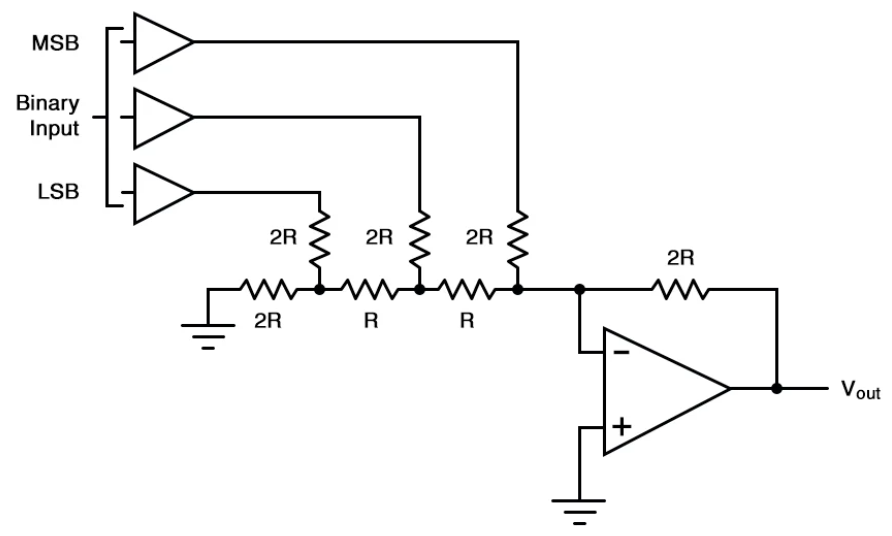
\includegraphics[scale = 0.4]{Figures/dac.png}
        \caption{$R/2R$ ladder DAC circuit}
        \label{fig:DAC}
    \end{figure}
    Output voltage of the DAC circuit is given by
    \begin{equation}
        V_{out} = -\dfrac{R_F}{R}\Bigg( \dfrac{d_1}{2^1} +\dfrac{d_2}{2^2}+\dfrac{d_3}{2^3} \Bigg)
    \end{equation}
    where $d_1$ is MSB (most significant bit) and $d_3$ is LSB (least significant bit) In the above circuit, feedback resistance $R_F = 2R$.
    \begin{table}[]
    \caption{Results of Digital-to-Analog converter circuit}
    \label{tab:DAC}
    \begin{tabular}{@{}cccc@{}}
    \toprule
    \multicolumn{2}{c}{\textbf{Digital Input}} & \begin{tabular}[c]{@{}c@{}}\textbf{Analog output}\\ (in volts, observed)\end{tabular} & \begin{tabular}[c]{@{}c@{}}\textbf{Analog output}\\ (in volts, theoretical)\end{tabular} \\ \midrule
    0 & 000 & 0.007 & 0 \\
    1 & 001 & -1.261 & -1.25 \\
    2 & 010 & -2.506 & -2.50 \\
    3 & 011 & -3.774 & -3.75 \\
    4 & 100 & -5.00 & -5.00 \\
    5 & 101 & -6.26 & -6.25 \\
    6 & 110 & -7.51 & -7.50 \\
    7 & 111 & -8.78 & -8.75 \\ \bottomrule
    \end{tabular}
    \end{table}
    \begin{figure}
        \centering
        \begin{subfigure}[b]{0.3\textwidth}
            \centering
            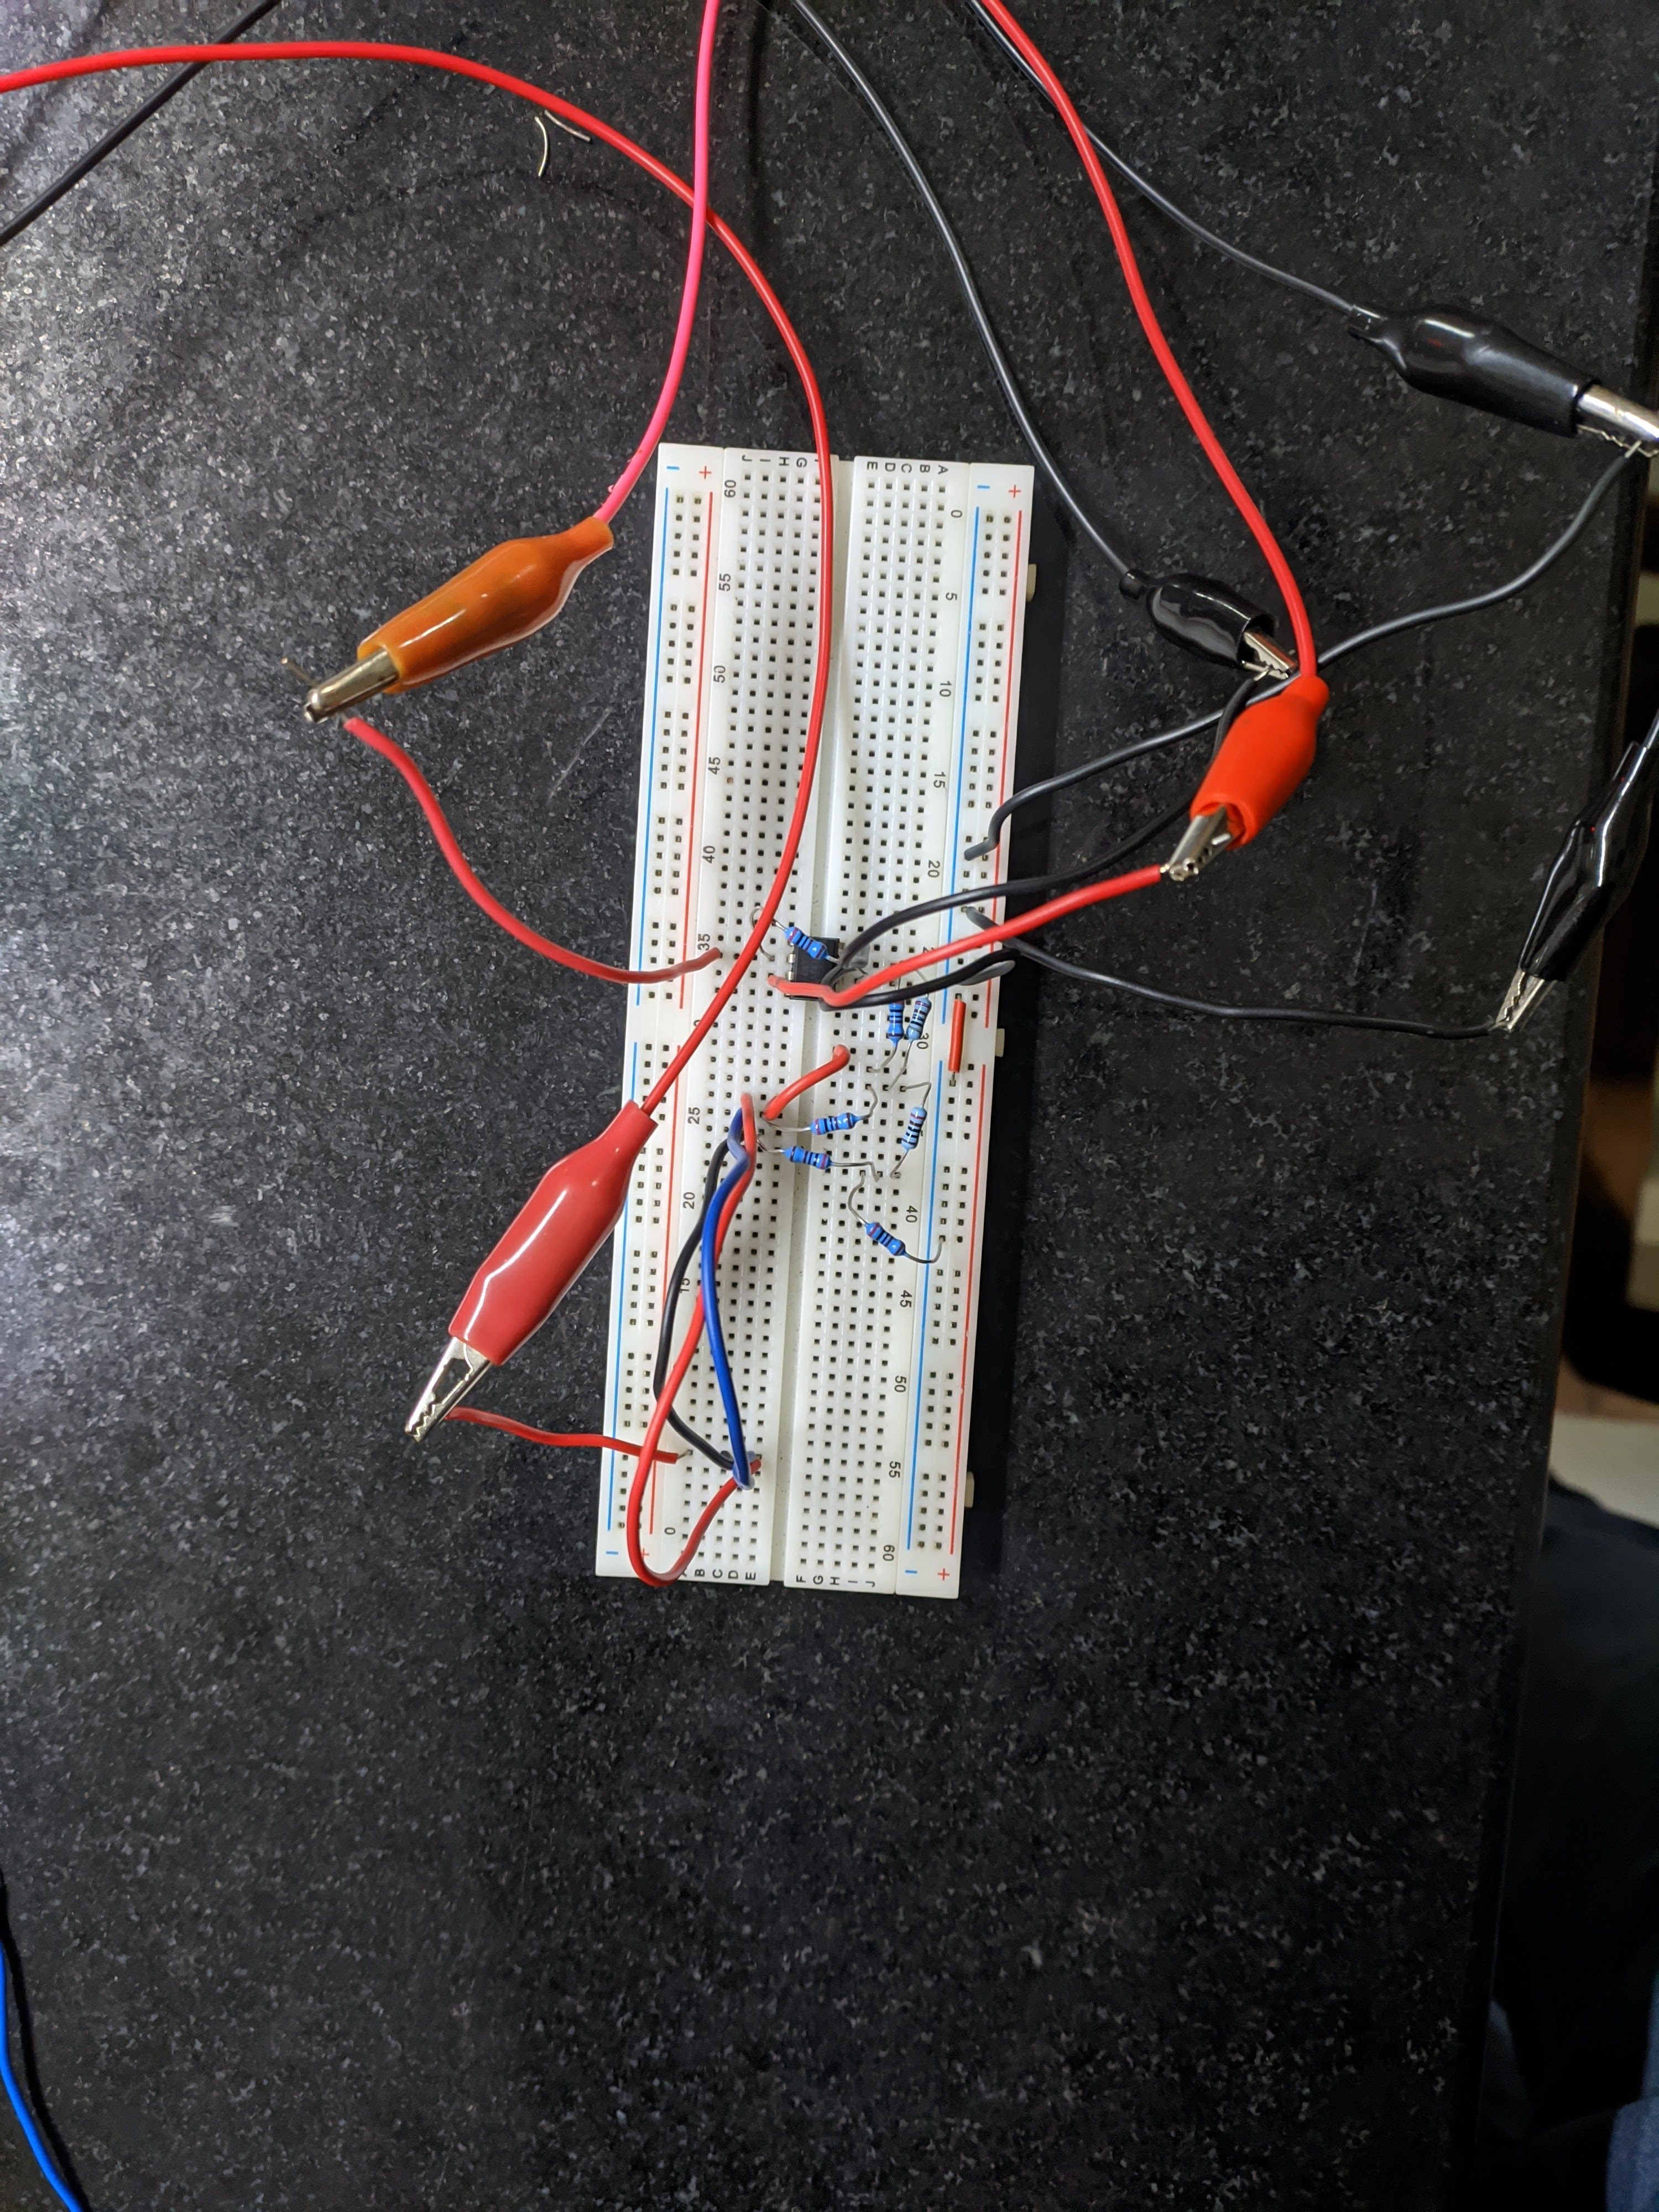
\includegraphics[width=\textwidth]{Figures/1.jpg}
            \caption{Top view}
            \label{fig:y equals x}
        \end{subfigure}
        \hfill
        \begin{subfigure}[b]{0.3\textwidth}
            \centering
            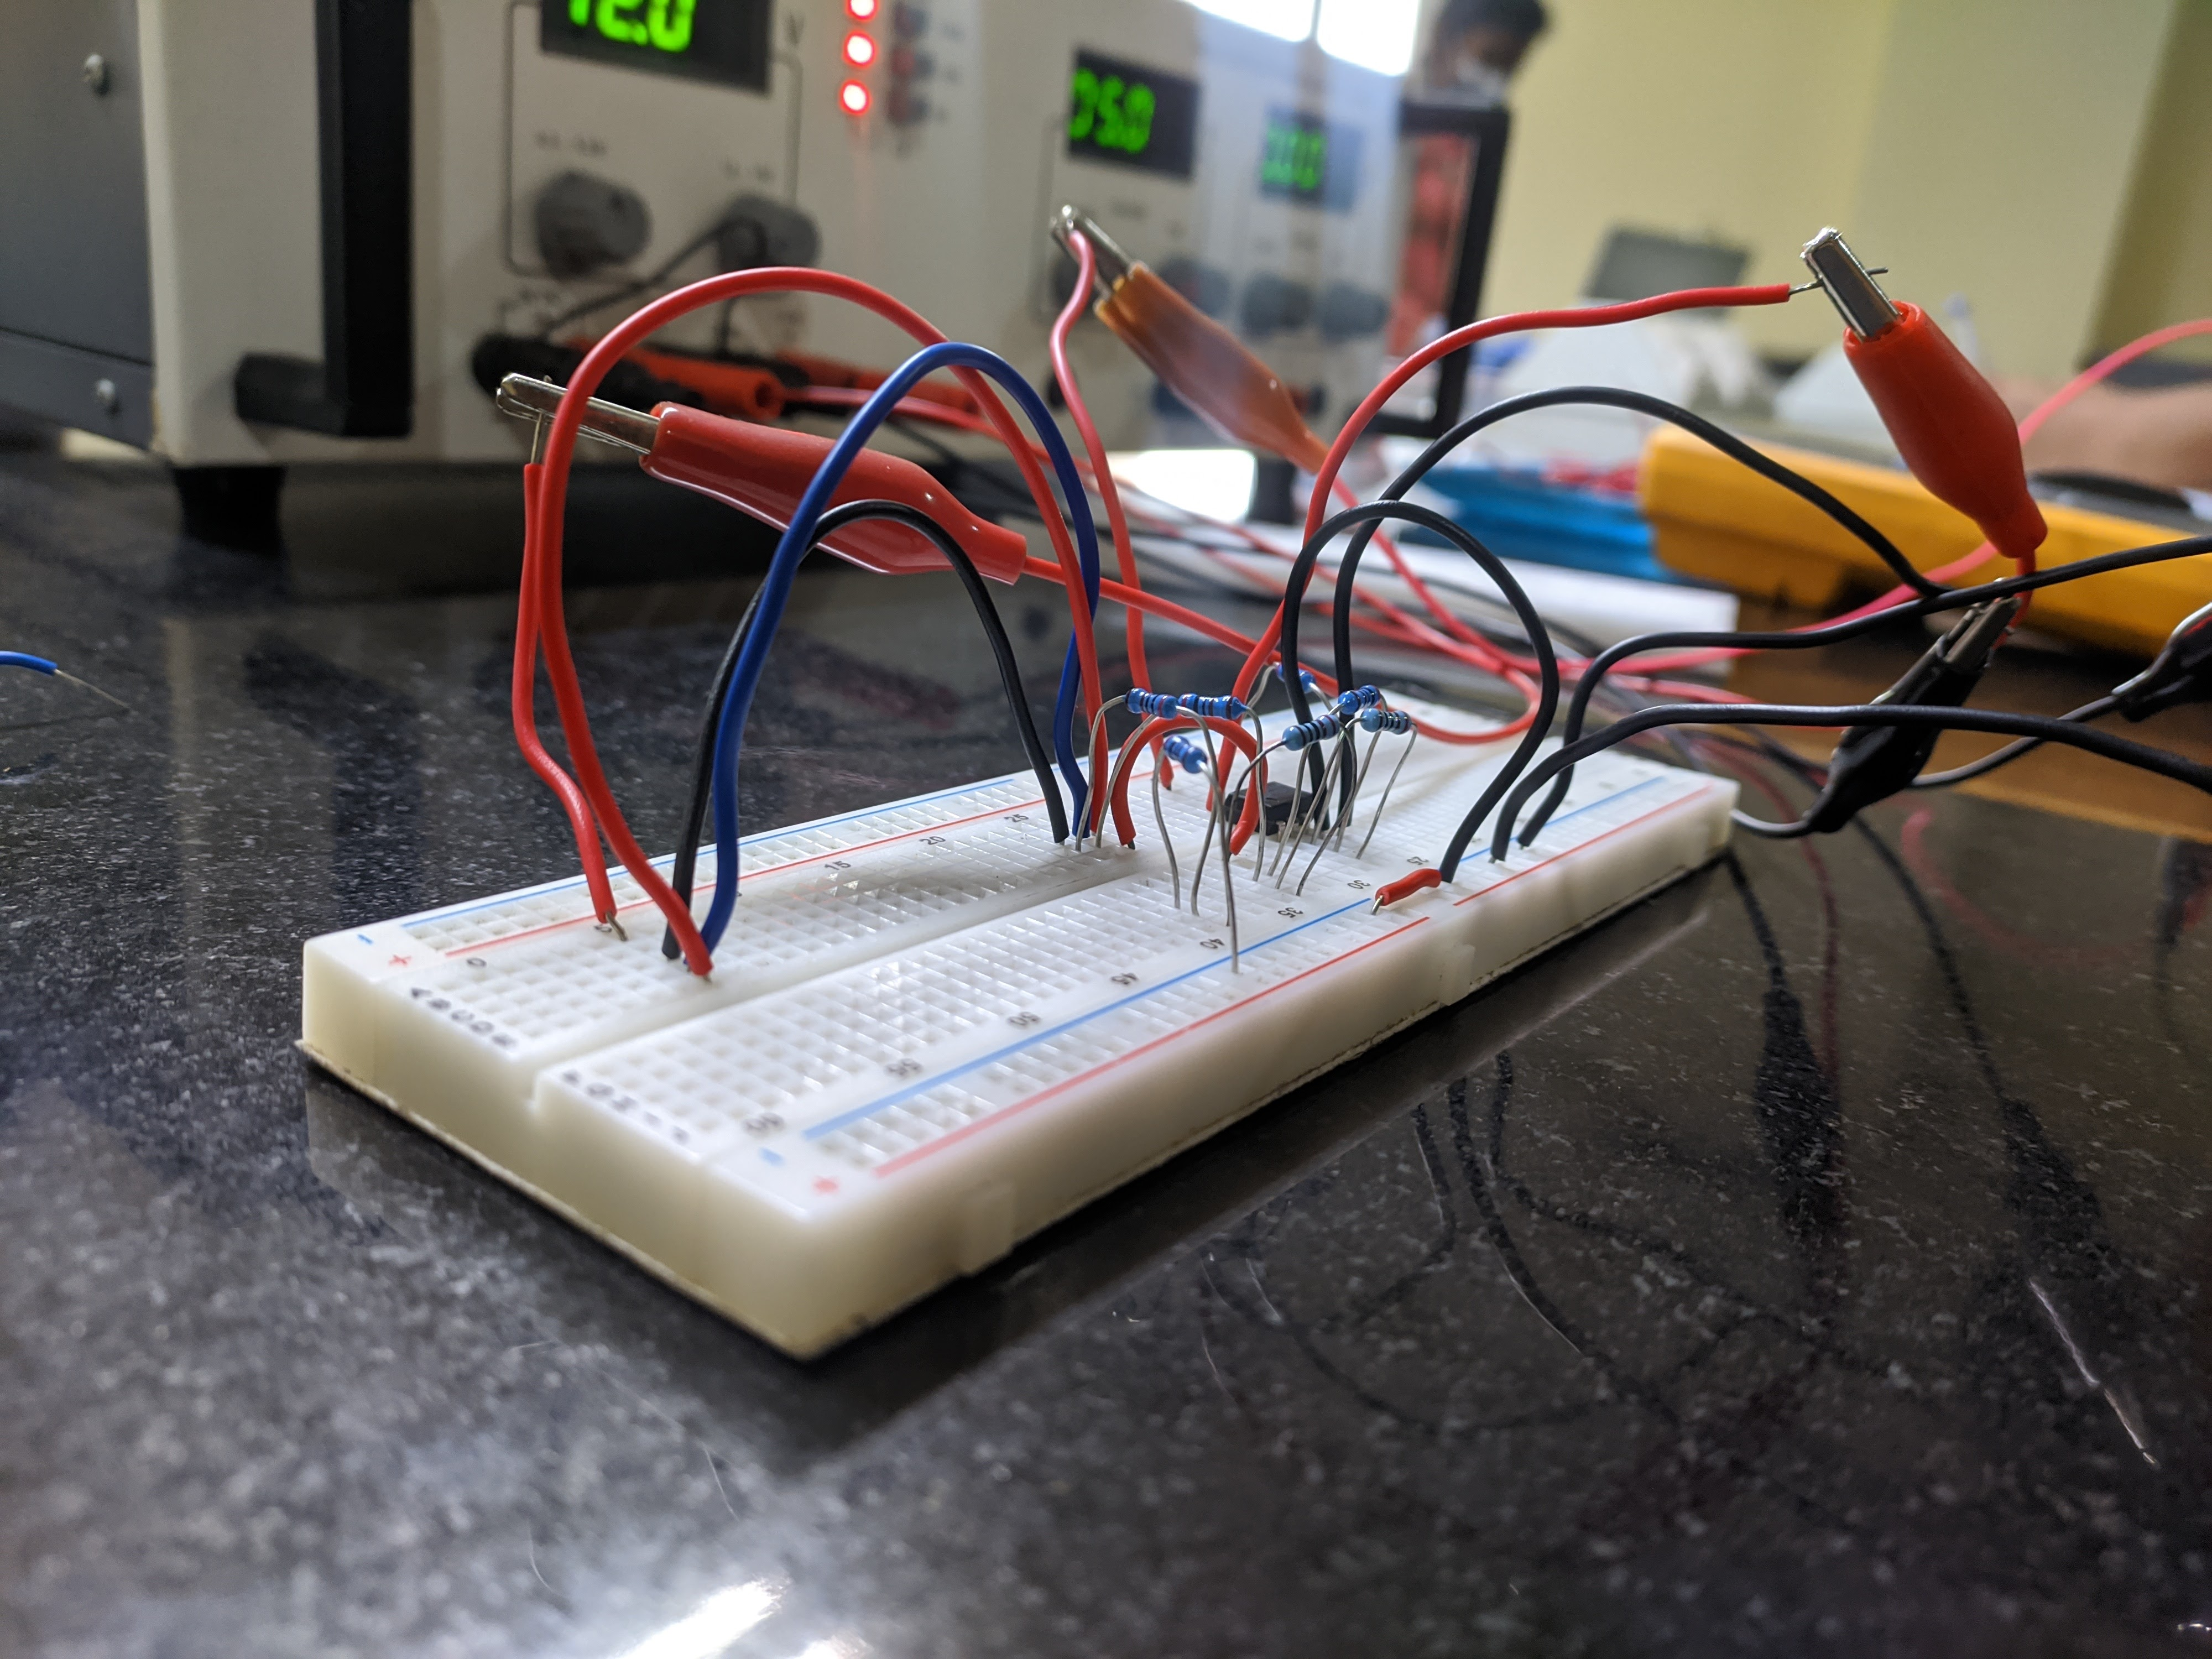
\includegraphics[width=\textwidth]{Figures/2.jpg}
            \caption{Side view}
            \label{fig:three sin x}
        \end{subfigure}
        \caption{Digital-to-Analog circuit}
    \end{figure}

\section{Analog-to-Digital converter}
    For the ADC, we will be employing the use of a \textit{flash ADC}. It is a type of analog-to-digital converter that uses a linear voltage ladder with a comparator at each \textit{rung} of the ladder to compare the input voltage to successive reference voltages. Often these reference ladders are constructed of many resistors; however, modern implementations show that capacitive voltage division is also possible. The output of these comparators is generally fed into a digital encoder, which converts the inputs into a binary value (the collected outputs from the comparators can be thought of as a unary value).
    \par
    It is formed of a series of comparators, each one comparing the input signal to a unique reference voltage. The comparator outputs connect to the inputs of a priority encoder circuit, which then produces a binary output.
    \par
    As the analog input voltage exceeds the reference voltage at each comparator, the comparator outputs will sequentially saturate to a high state. The priority encoder generates a binary number based on the highest-order active input, ignoring all other active inputs.
    \par
    When operated, the flash ADC produces an output that looks something like shown in figure (\ref{fig:flashadc}).
    \begin{figure}
        \centering
        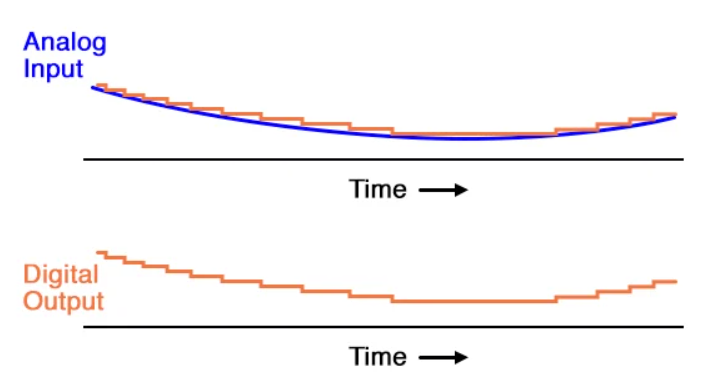
\includegraphics[scale = 0.55]{Figures/flashadc.png}
        \caption{Output of a flash ADC circuit}
        \label{fig:flashadc}
    \end{figure}
    Not only is the flash converter the simplest in terms of operational theory, but it is the most efficient of the ADC technologies in terms of speed, being limited only in comparator and gate propagation delays. Unfortunately, it is the most component-intensive for any given number of output bits.
    \par
    With equal-value resistors in the reference voltage divider network, each successive binary count represents the same amount of analog signal increase, providing a proportional response. For special applications, however, the resistor values in the divider network may be made non-equal.
    \par
    This gives the ADC a custom, nonlinear response to the analog input signal. No other ADC design is able to grant this signal-conditioning behavior with just a few component value changes.
    \subsection{Working}
    \begin{figure}
        \centering
        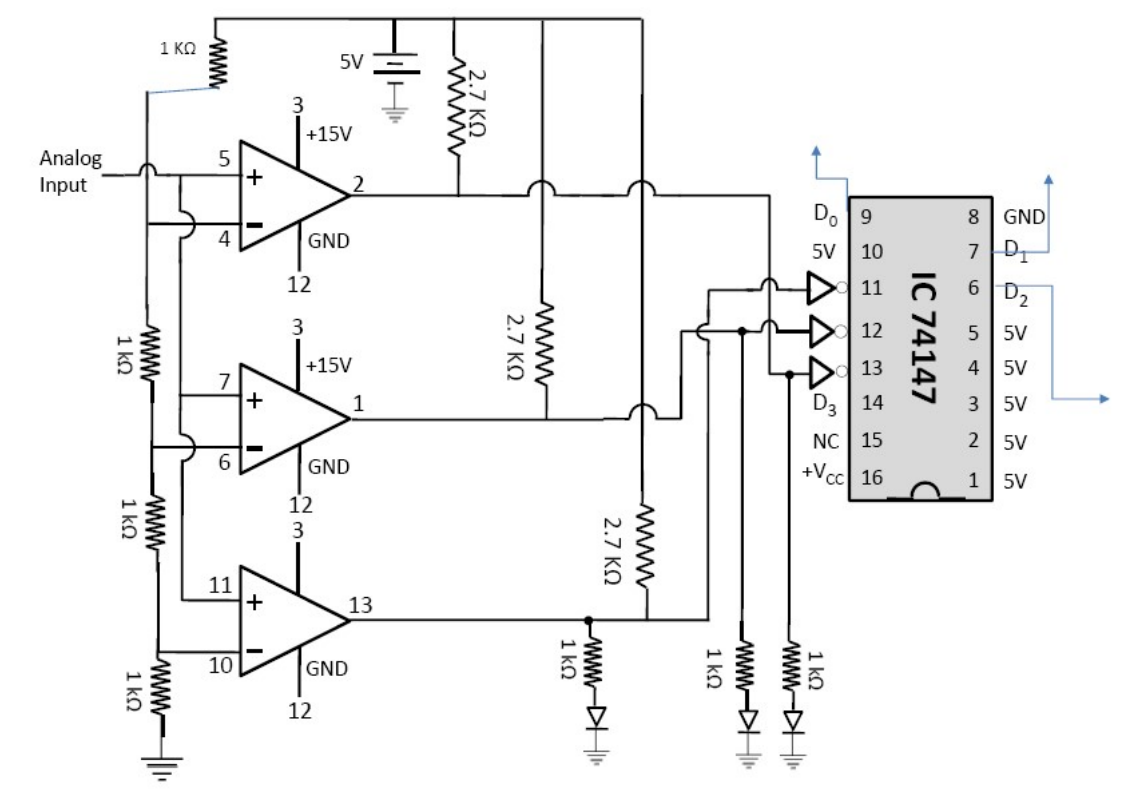
\includegraphics[scale = 0.35]{Figures/adc.png}
        \caption{Circuit diagram for 2-bit binary Analog-to-Digital conversion}
        \label{fig:ADC}
    \end{figure}
    Analog input from the DC power supply is compared with reference voltage using LM339 comparator chip and then given to 74LS147 priority encoder chip. Binary output obtained from 74LS147 further can be converted to BCD format using 7447 chip, which can displayed on common cathode 7-segment BCD display as decimal digit.
    \par
    We use three out of four comparators available in LM339. IC pin diagrams of LM339 and IC 74147 are given figures (\ref{fig:339}) and (\ref{fig:7447}) respectively. Digital binary output can be obtained from $D_0$, $D_1$ and $D_2$ or pin nos. 9, 7 and 6 of IC 74147.
    \subsection{Components}
    \begin{figure}
        \centering
        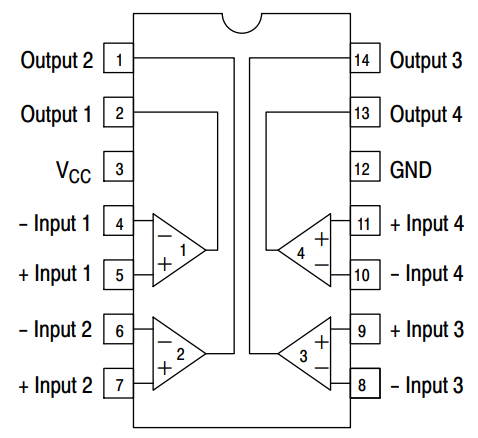
\includegraphics[scale = 0.60]{Figures/lm339.png}
        \caption{Pin diagram for the LM339 comparator}
        \label{fig:339}
    \end{figure}
    LM339 (figure (\ref{fig:339})) is a quad comparator integrated circuit. It has open collector, therefore requires pull up resistors as shown in figure (\ref{fig:ADC}) at the output of comparator. Pull up resistors of $\SI{3}{\kilo \ohm}$ are used. $\SI{1}{\kilo \ohm}$ resistors are used in series with the LEDs while using LM339 chip. Supply voltage to LM339 can be up to 15 V. The supply voltage must be set appropriately. It is essential to ensure the correct working of the comparator circuit before connecting the NOT gates and LEDs for digital output.
    \begin{figure}
        \centering
        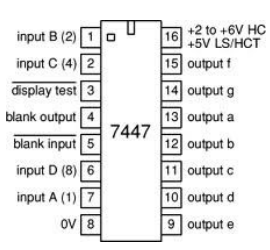
\includegraphics[scale = 1]{Figures/real7447.png}
        \caption{Pin diagram for the IC7447 priority encoder}
        \label{fig:7447}
    \end{figure}
    \par
    74LS147 is 10 to 4 priority encoder. For this IC, input is active low and output is active low. Pin diagram is given in figure (\ref{fig:7447}). Unused input pins of 74147 should not be left open and they need to be connected to 5 V input supply.

    \begin{table}[]
    \caption{Results of Digital-to-Analog converter circuit}
    \label{tab:ADC}
    \setlength{\tabcolsep}{15pt}
    \begin{tabular}{@{}ccc@{}}
    \toprule
    \multirow{2}{*}{\textbf{Analog input} (volts)} & \multicolumn{2}{c}{\textbf{Digital output}} \\ \cmidrule(l){2-3} 
     & $D_0$ & $D_1$ \\ \midrule
    0 & 0 & 0 \\
    1.3 & 0 & 1 \\
    2.5 & 1 & 0 \\
    3.8 & 1 & 1 \\ \bottomrule
    \end{tabular}
    \end{table}
    \begin{figure}
        \centering
        \begin{subfigure}[b]{0.3\textwidth}
            \centering
            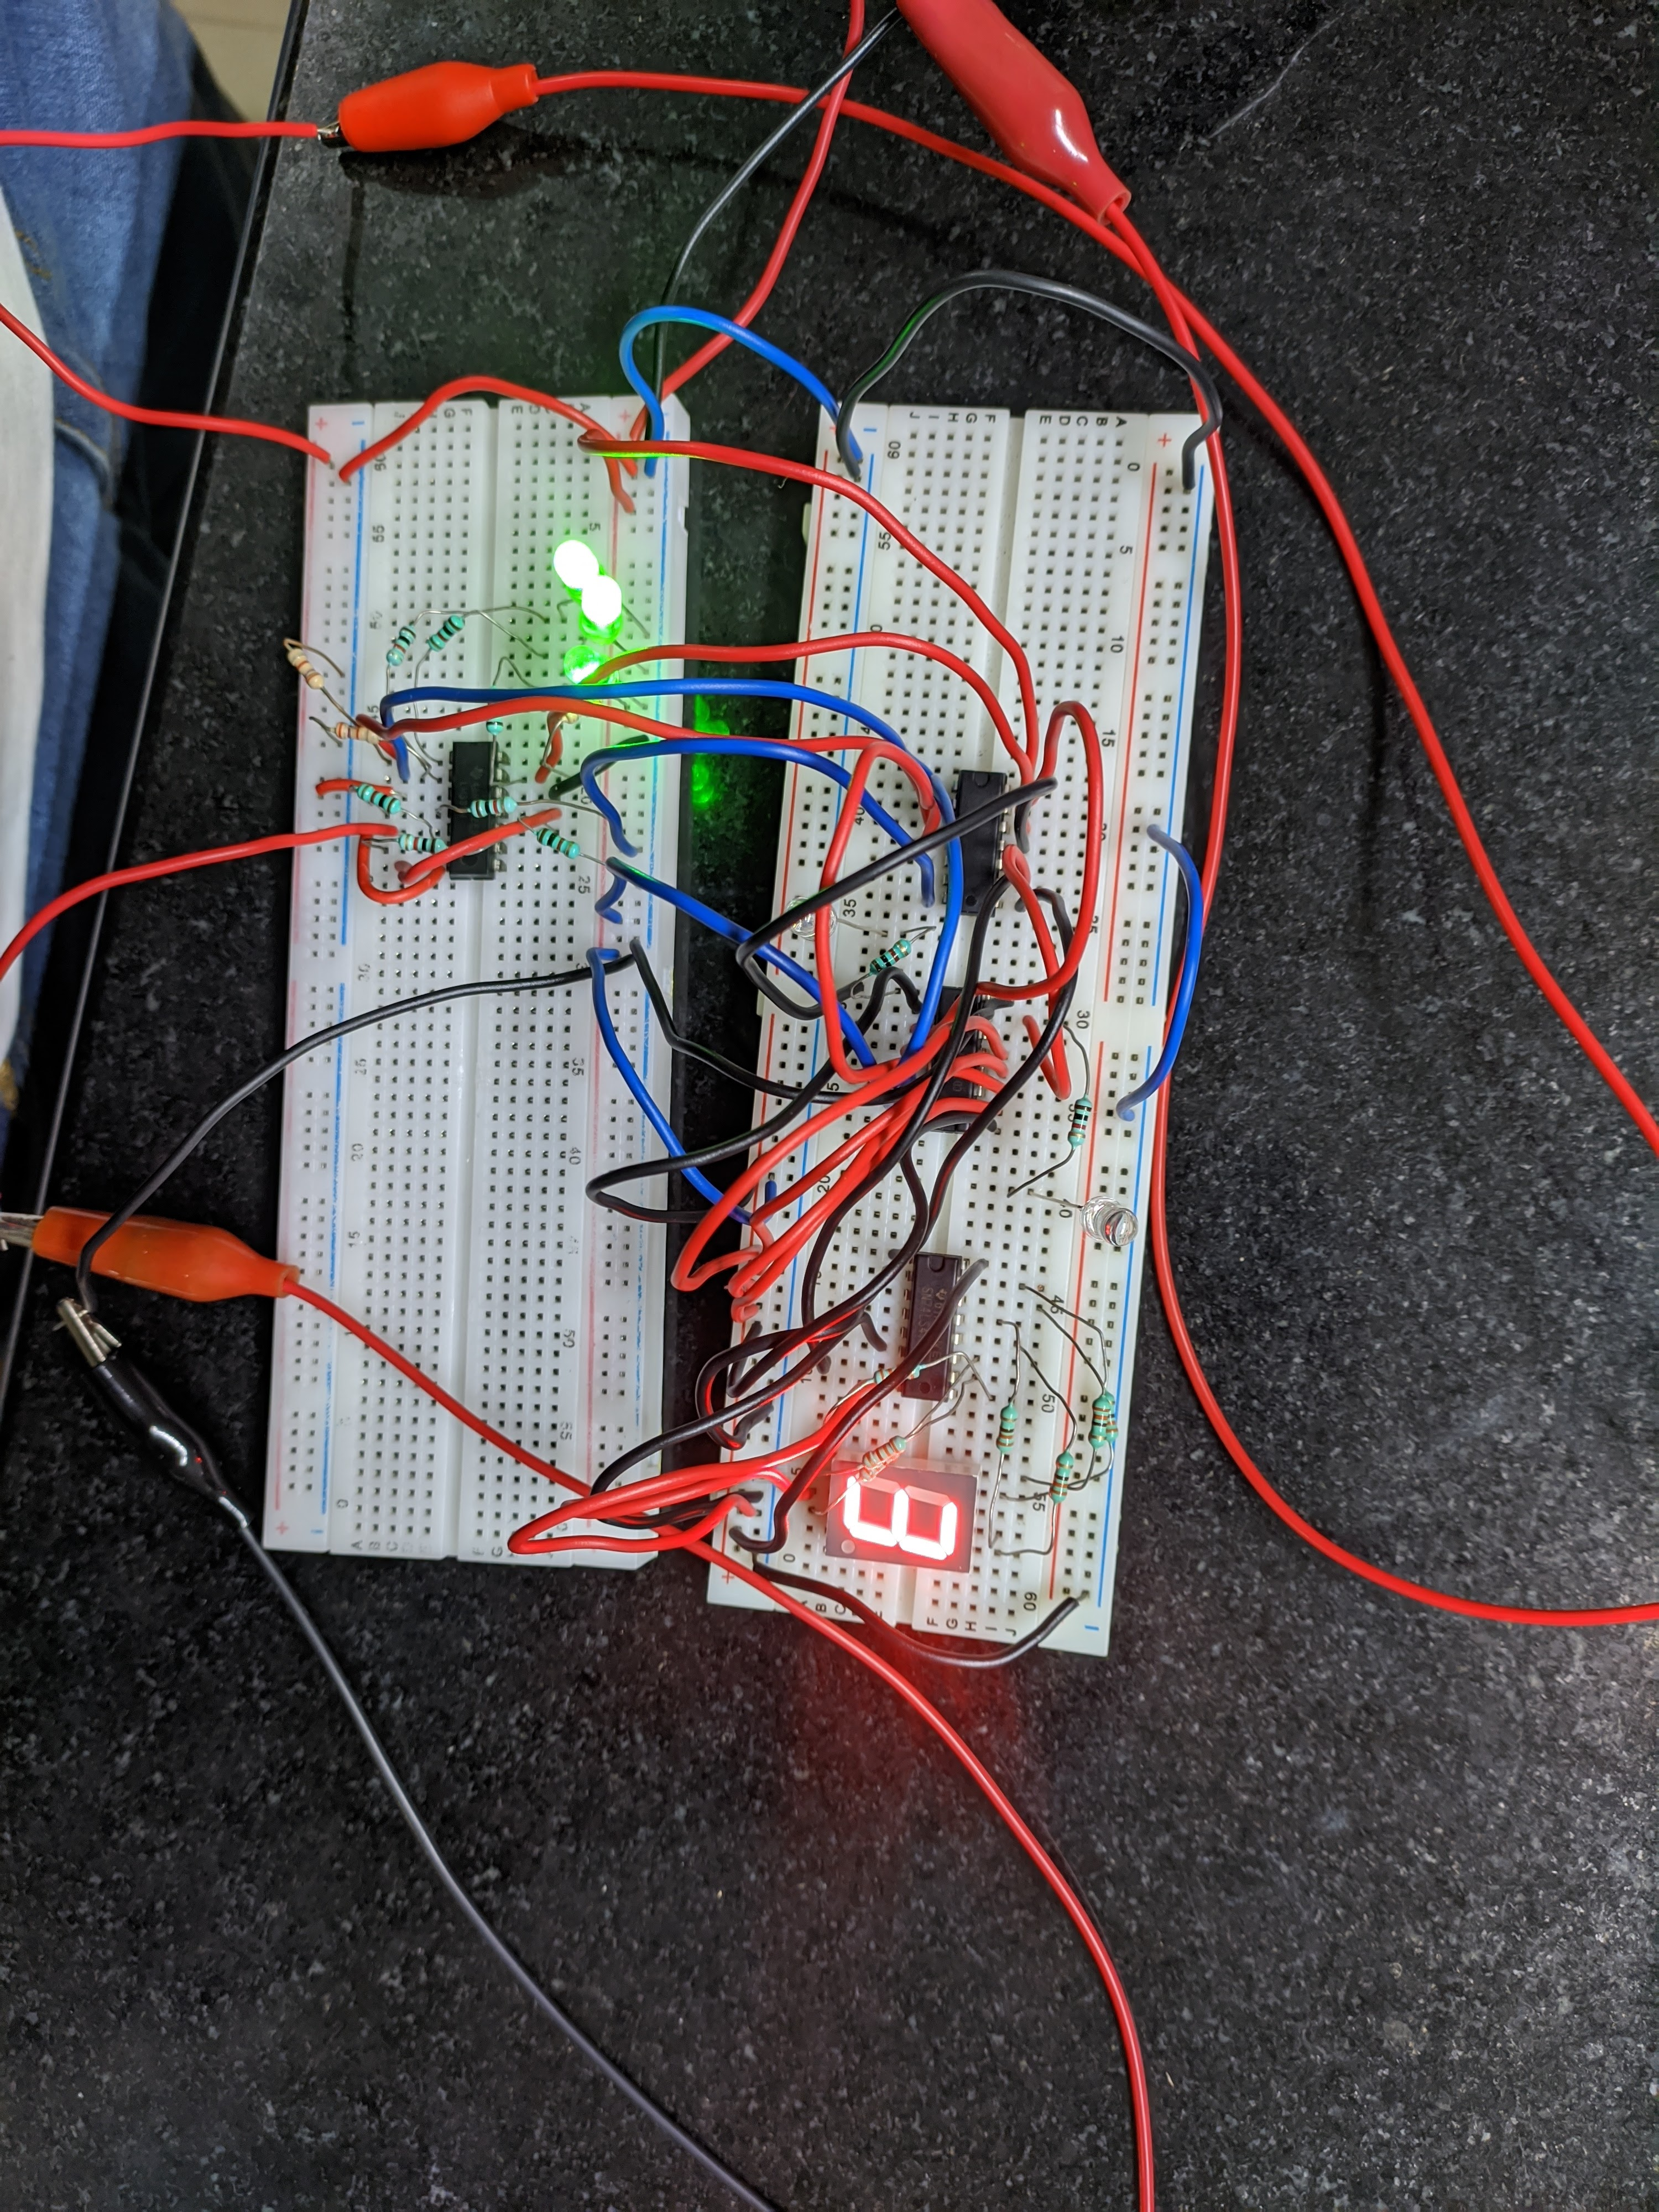
\includegraphics[width=\textwidth]{Figures/3.jpg}
            \caption{Top view}
            \label{fig:y equals x}
        \end{subfigure}
        \hfill
        \begin{subfigure}[b]{0.3\textwidth}
            \centering
            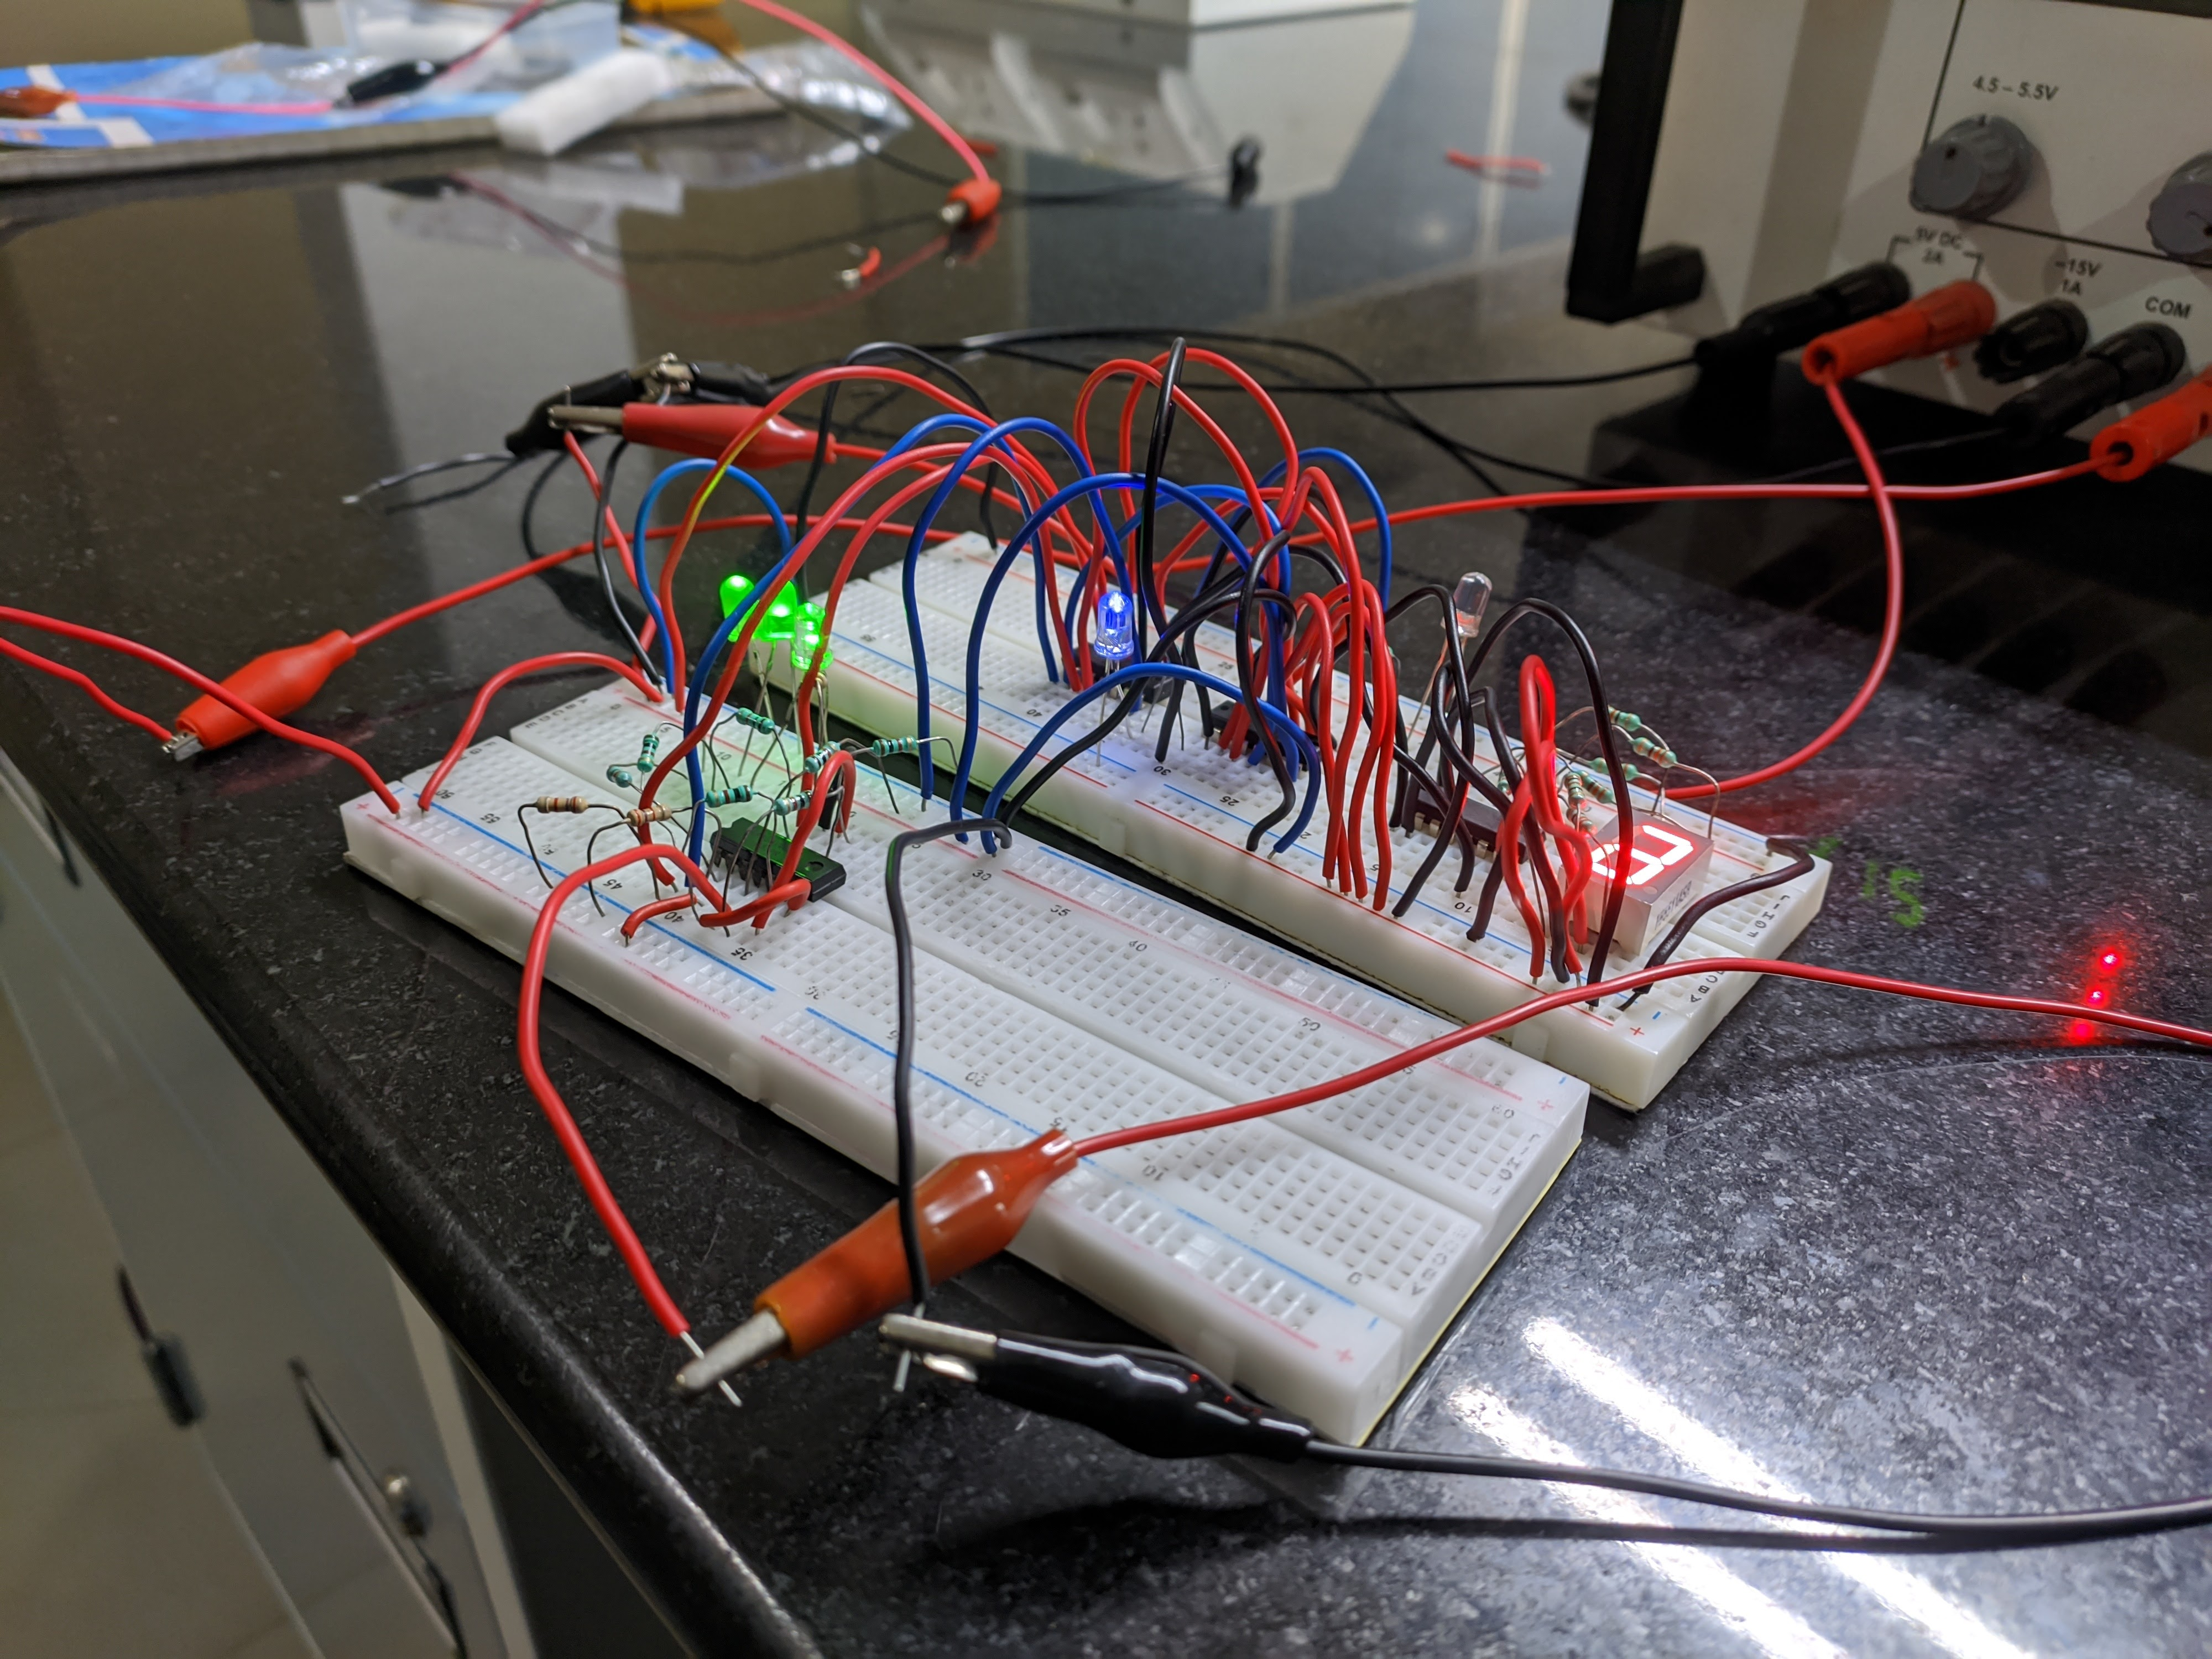
\includegraphics[width=\textwidth]{Figures/4.jpg}
            \caption{Side view}
            \label{fig:three sin x}
        \end{subfigure}
        \caption{Analog-to-Digital circuit}
    \end{figure}

\section{Conversion of Binary display to digital display}
    After converting analog voltage to binary number, further it can be converted to binary coded decimal and displayed on a BCD display. Pin diagram for 7447 (binary to BCD decoder) and common anode BCD display is given in figure (\ref{fig:bcd}). 7447 is an input active high IC and output active low IC. Output of the 7447 must be connected to BCD display via a $\SI{330}{\ohm}$ resistor. There are two types of BCDs. We use in the lab Common anode BCD display, which is input active low.
    \begin{figure}
        \centering
        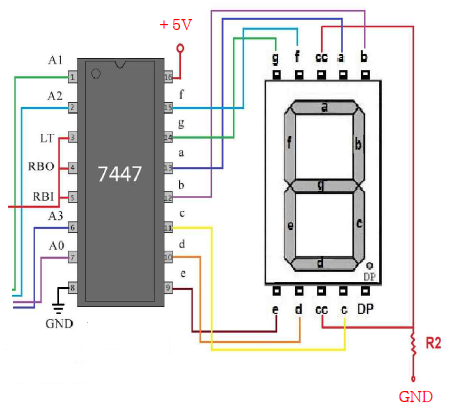
\includegraphics[scale = 0.85]{Figures/7447-decoder.png}
        \caption{Circuit diagram for IC7447 and 7-segment BCD display circuit}
        \label{fig:bcd}
    \end{figure}

    \begin{table}[]
    \caption{Results for the 7-segment BCD display circuit experiment}
    \label{tab:bcd}
    \setlength{\tabcolsep}{15pt}
    \begin{tabular}{@{}cc@{}}
    \toprule
    \textbf{Analog Input} & \textbf{BCD Display Output} \\ \midrule
    0 & 0 \\
    1.3 & 1 \\
    2.5 & 2 \\
    3.8 & 3 \\ \bottomrule
    \end{tabular}
    \end{table}
    \begin{figure}
        \centering
        \begin{subfigure}[b]{0.3\textwidth}
            \centering
            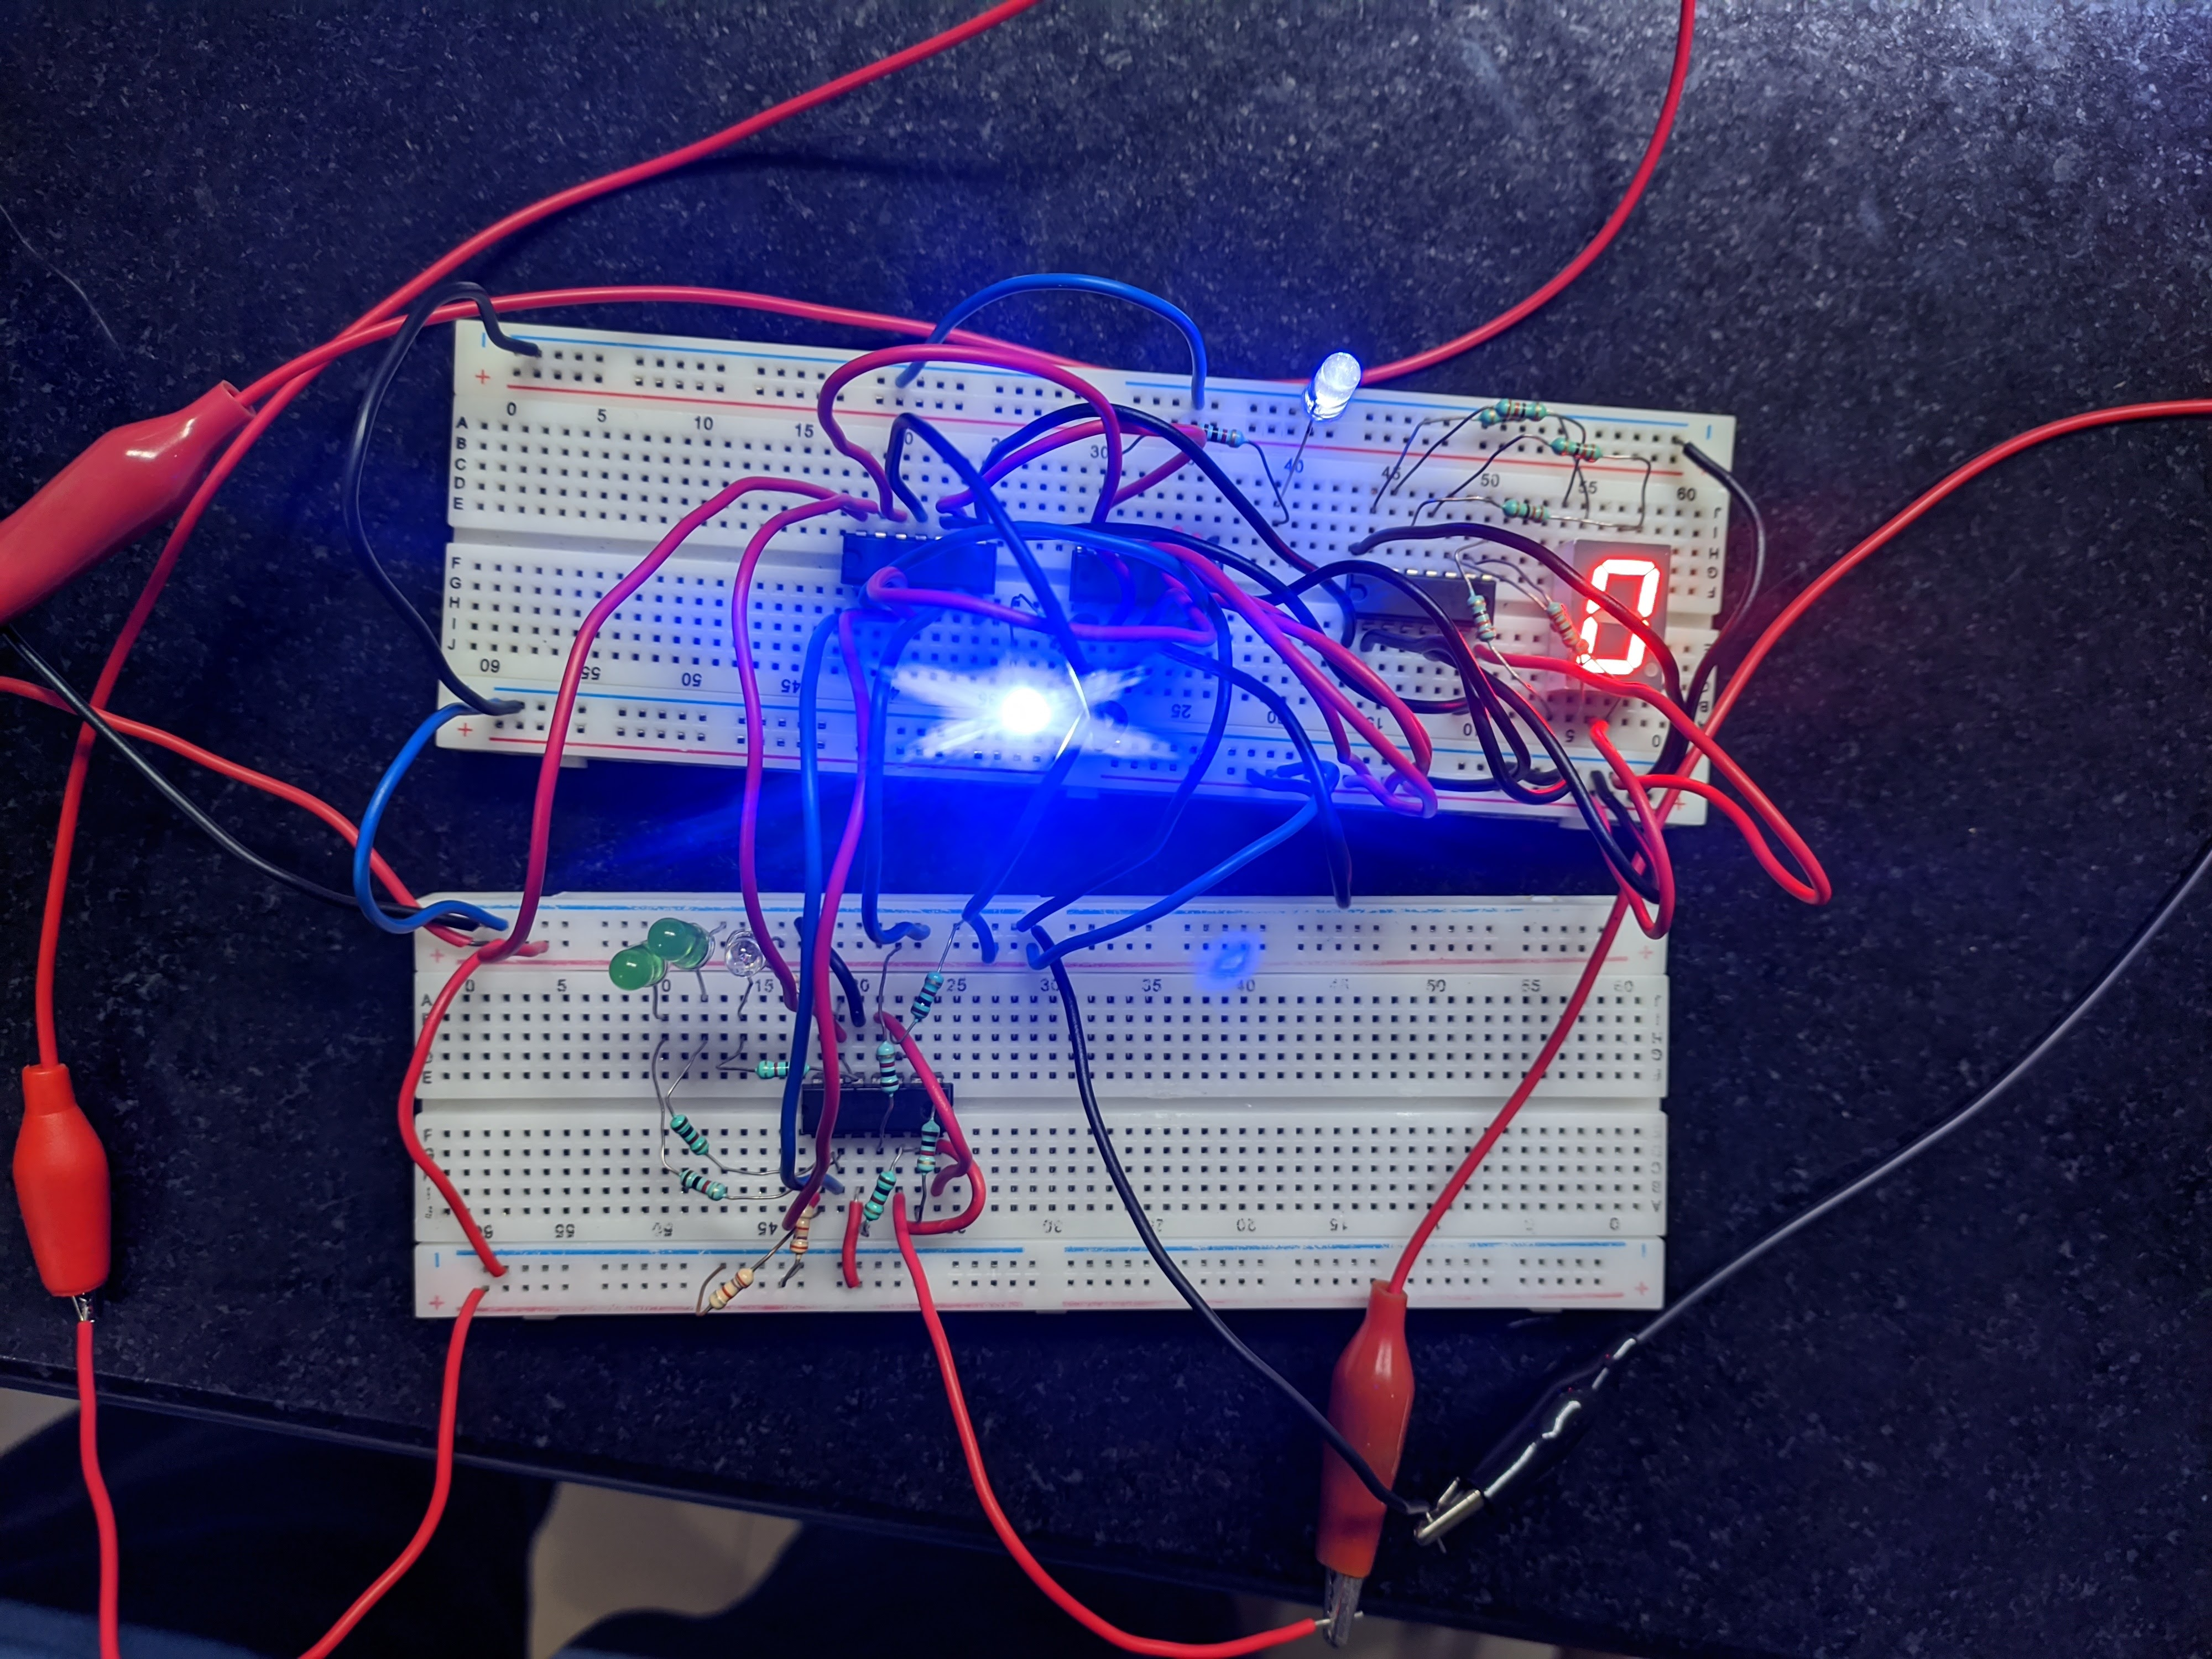
\includegraphics[width=\textwidth]{Figures/5.jpg}
            \caption{The BCD display reads 0}
            \label{fig:y equals x}
        \end{subfigure}
        \hfill
        \begin{subfigure}[b]{0.3\textwidth}
            \centering
            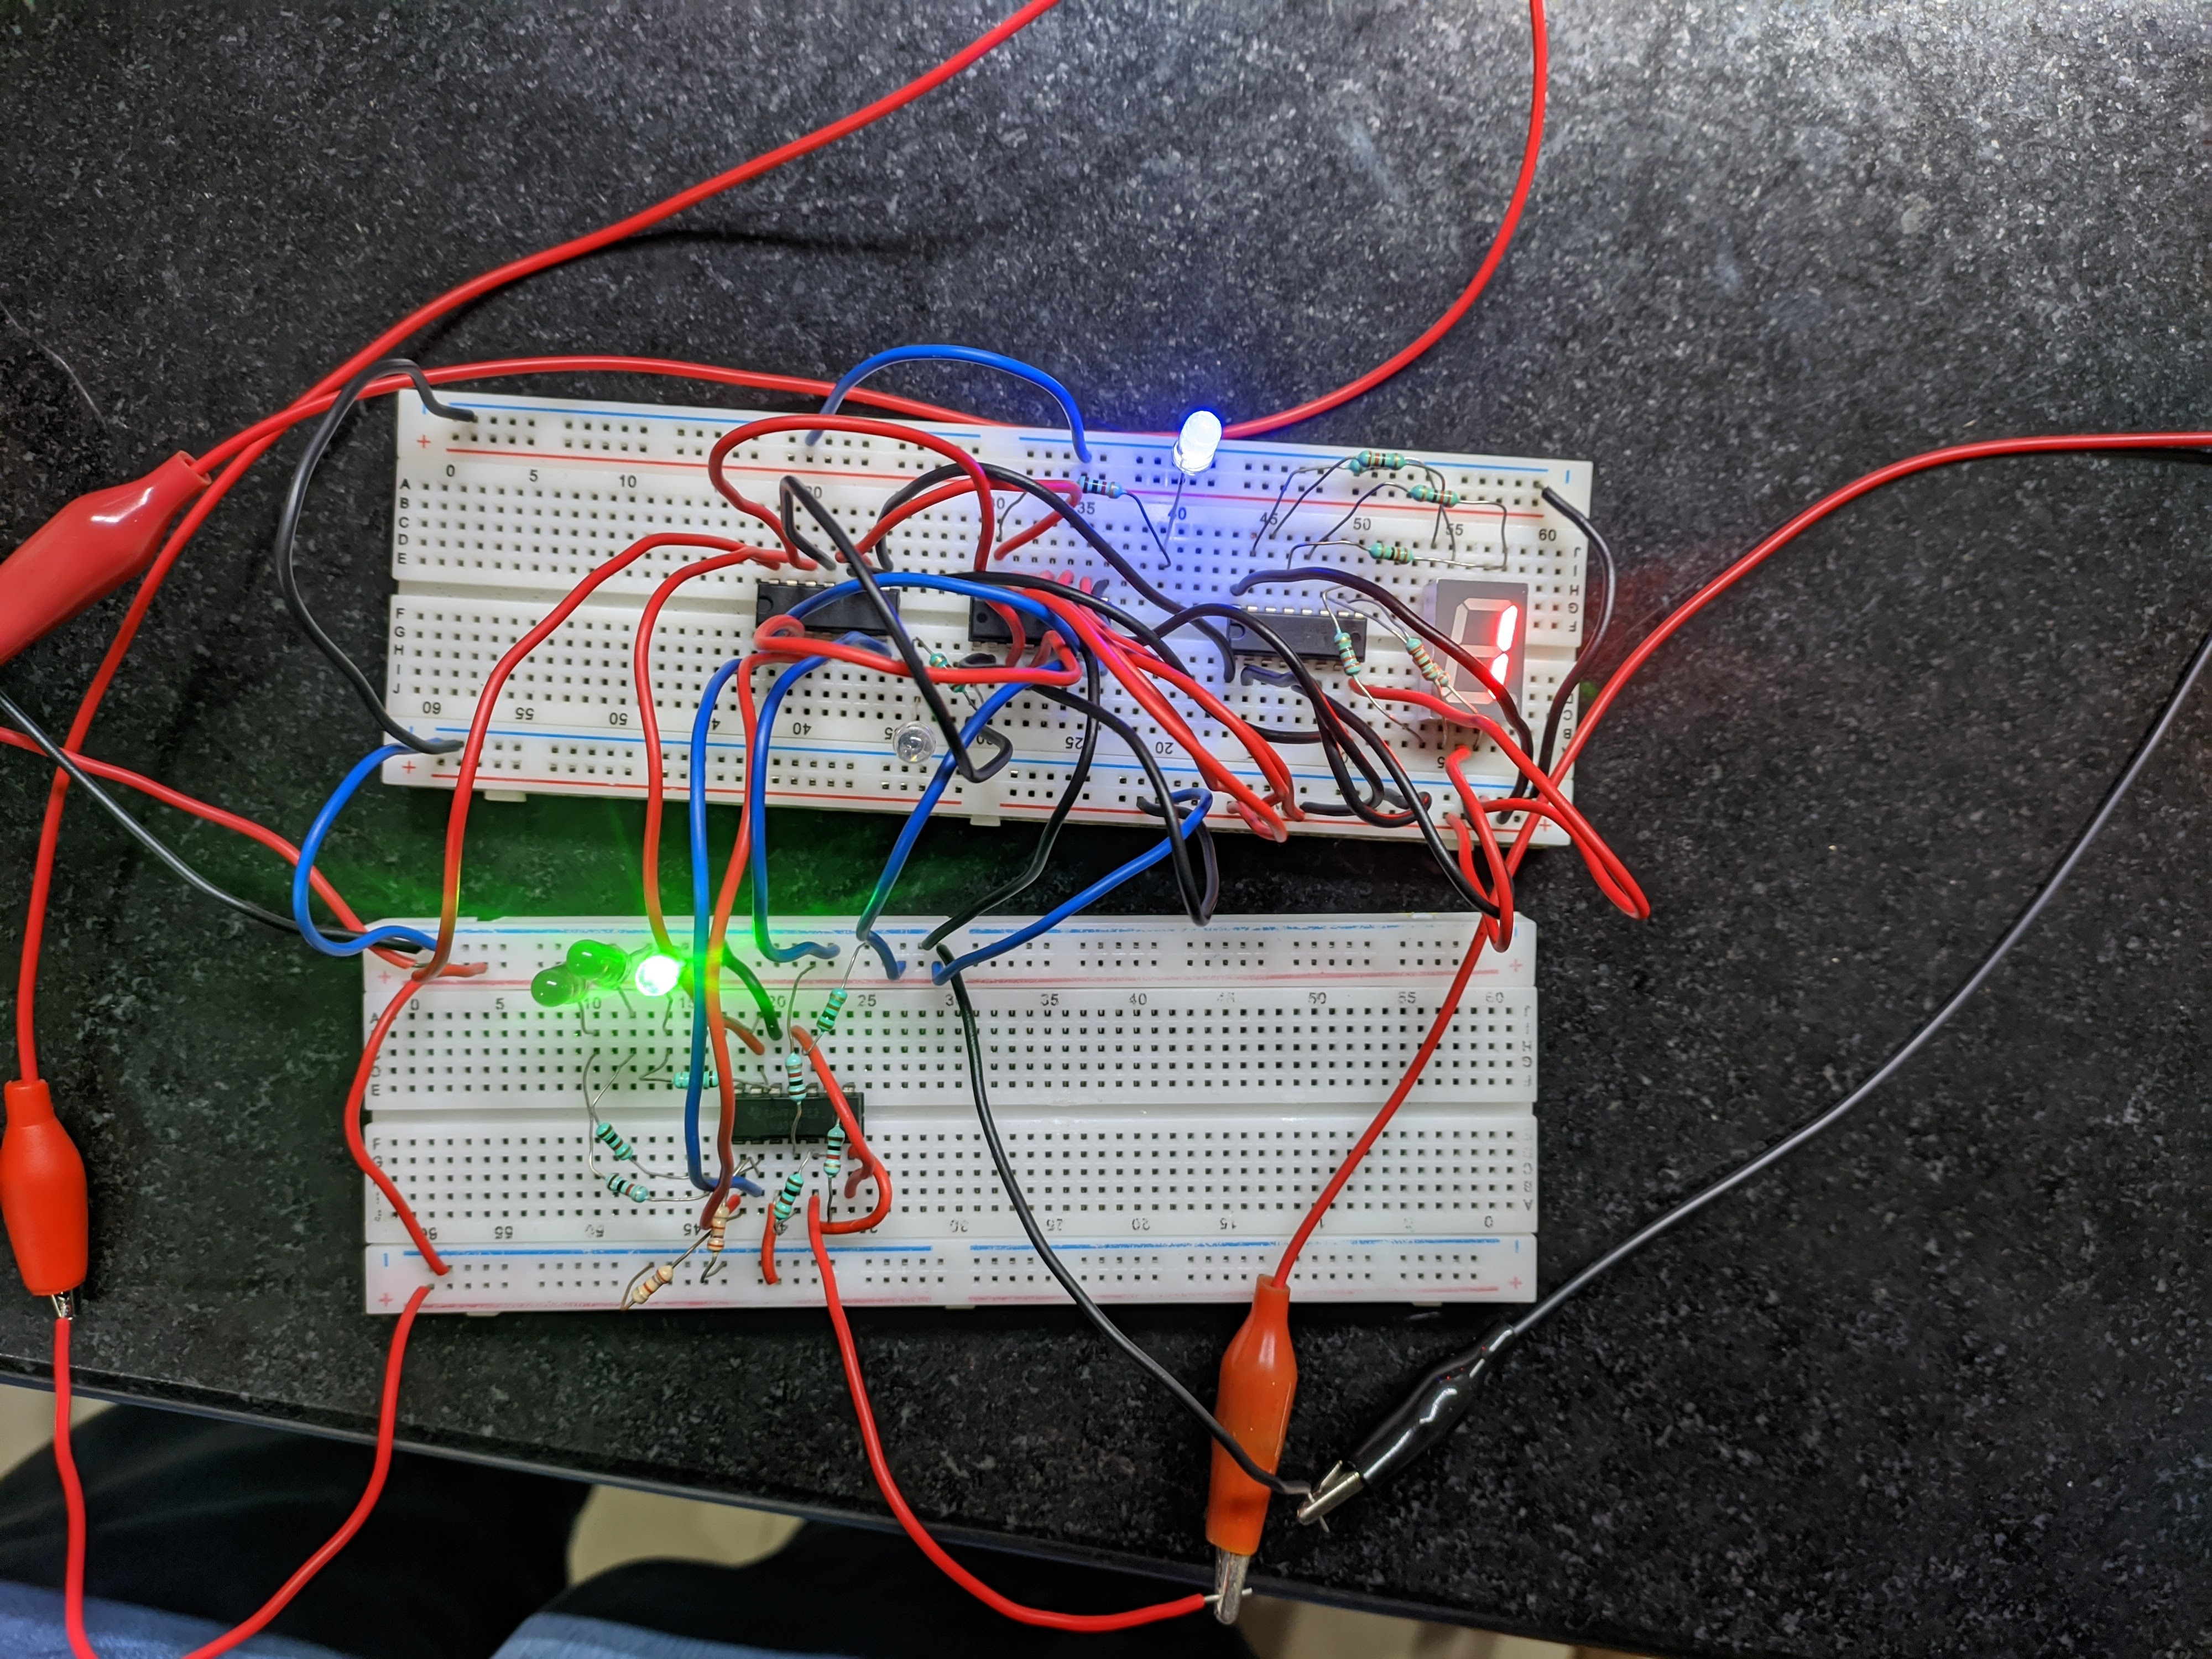
\includegraphics[width=\textwidth]{Figures/6.jpg}
            \caption{The BCD display reads 1}
            \label{fig:three sin x}
        \end{subfigure}
        \hfill
        \begin{subfigure}[b]{0.3\textwidth}
            \centering
            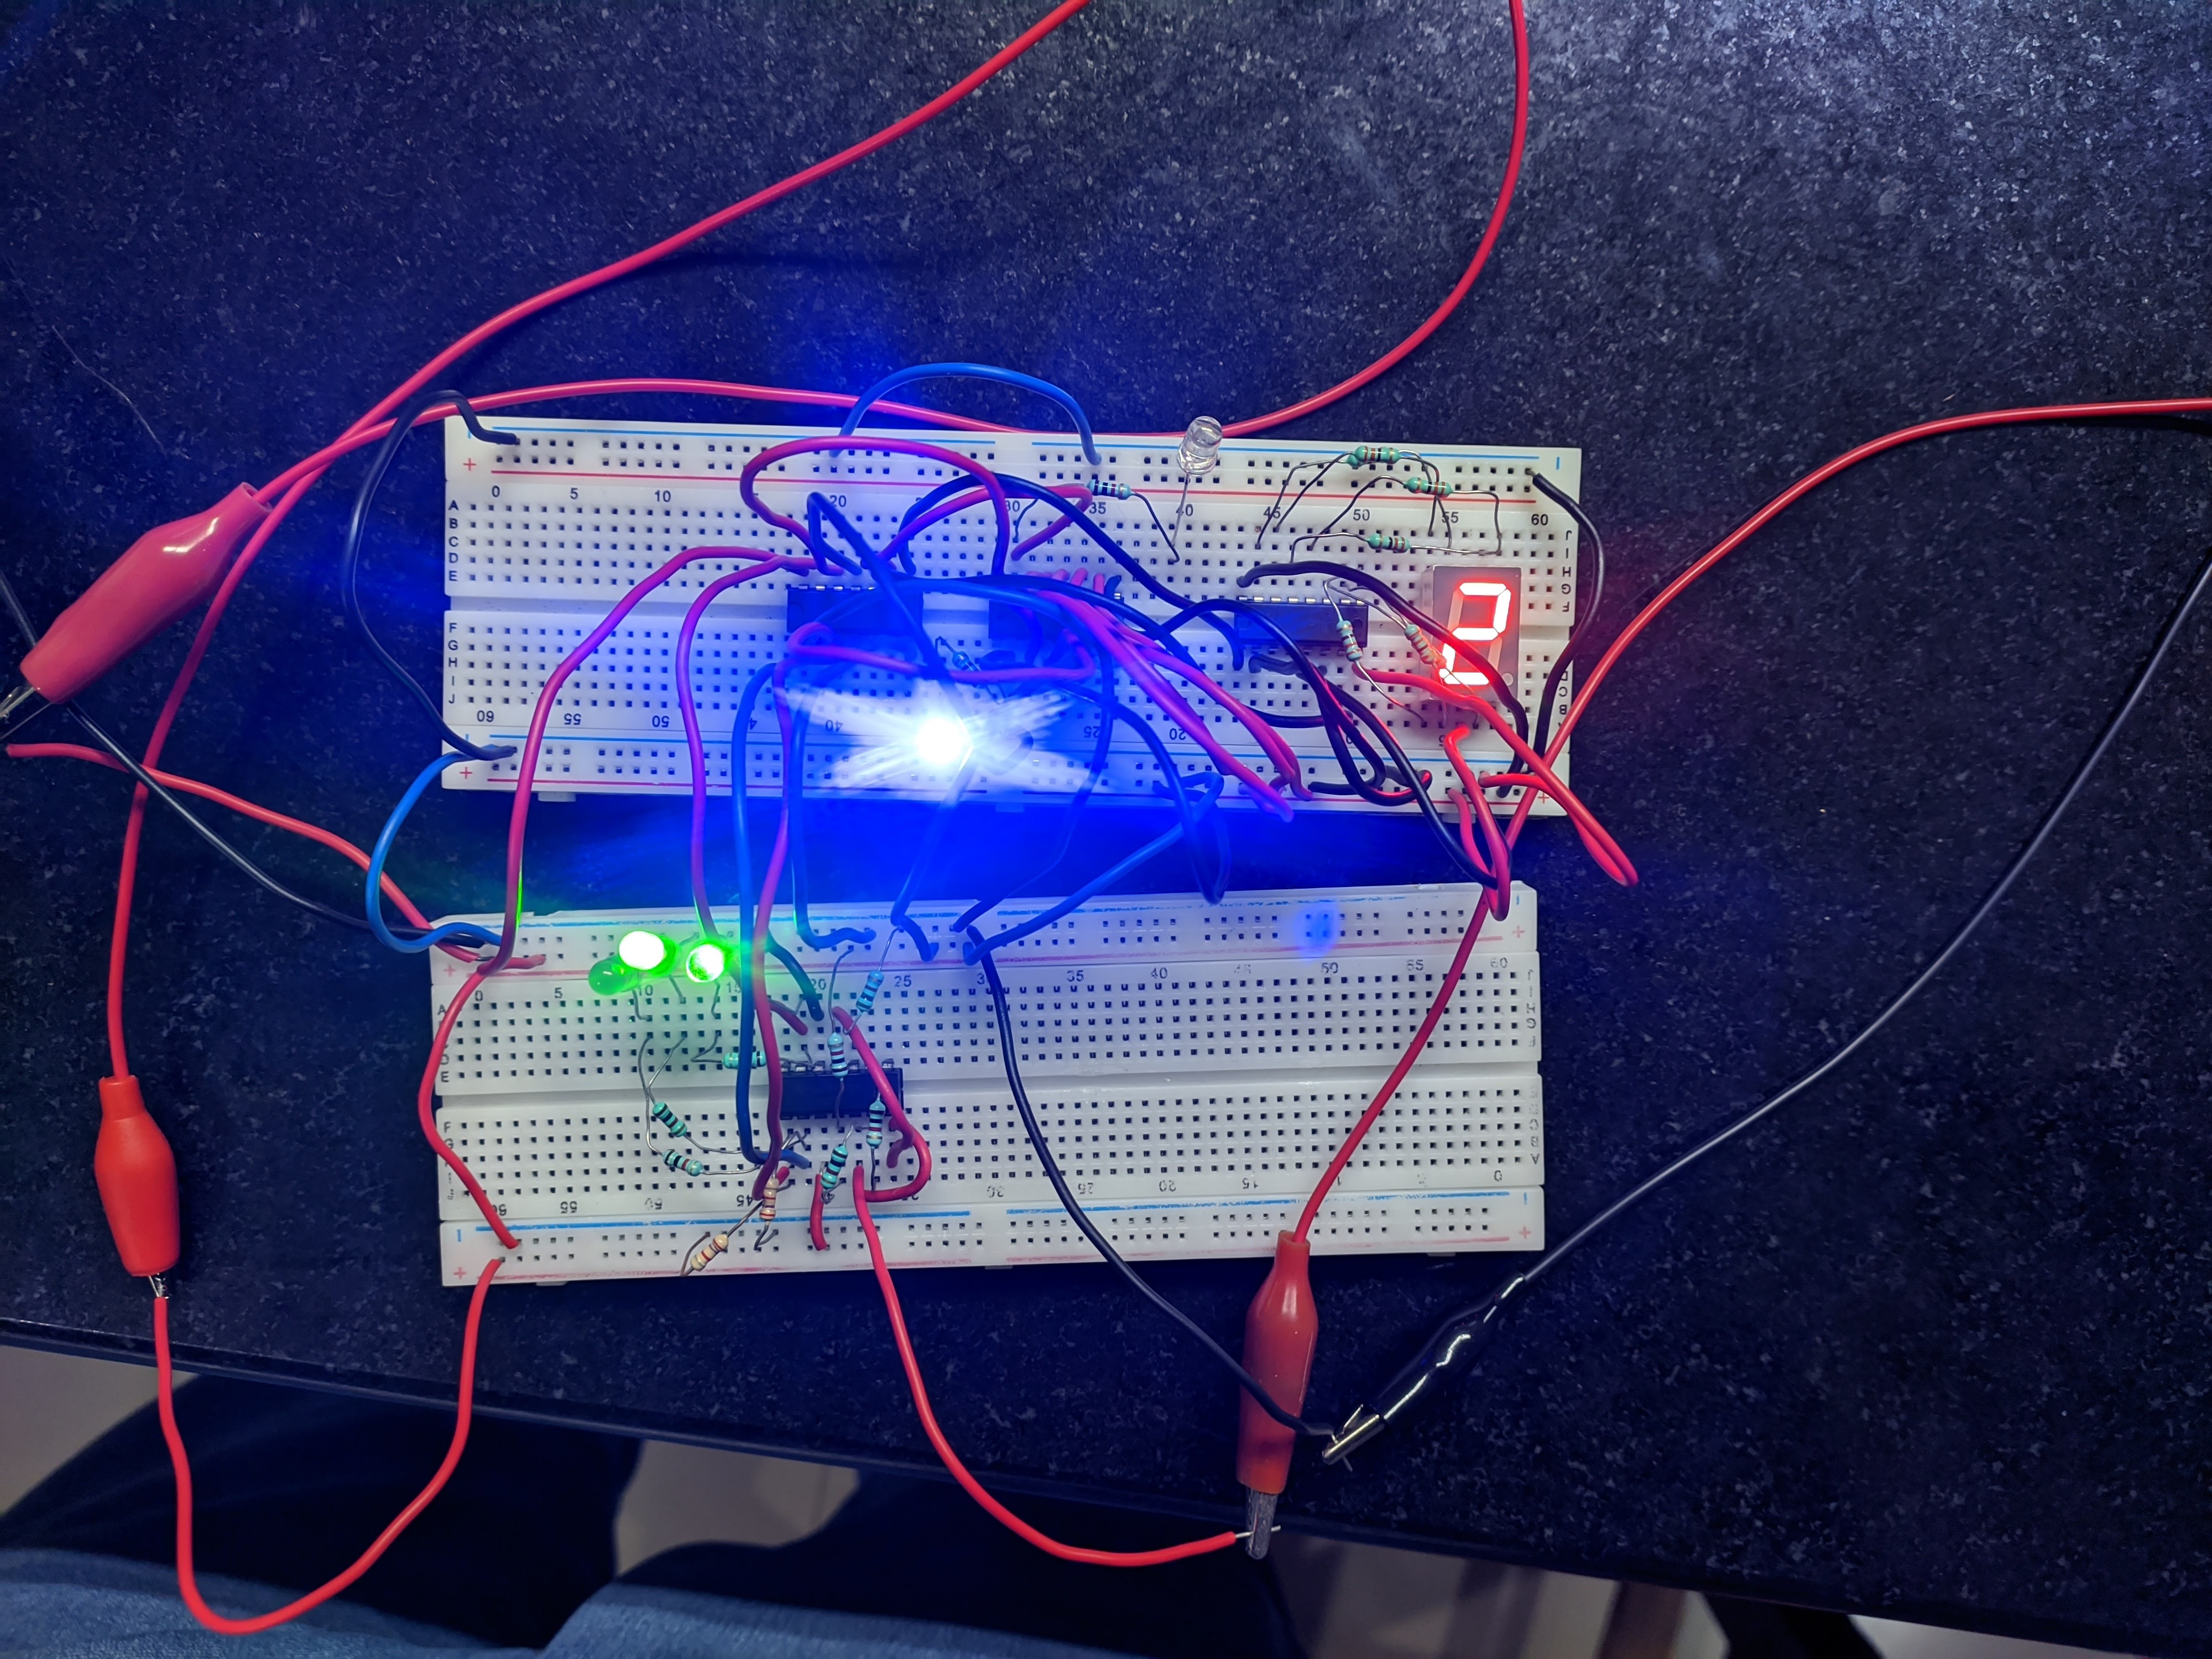
\includegraphics[width=\textwidth]{Figures/7.jpg}
            \caption{The BCD display reads 2}
            \label{fig:three sin x}
        \end{subfigure}
        \caption{Analog-to-Digital connected with a BCD display}
    \end{figure}
    
\section{Results}
    The verified (signed) results are appended at the end of this report. The results were as expected and in line with the theory.
    
\section{Discussions}
    \begin{enumerate}
        \item For the DAC circuit, we could have constructed a $R/128R$ ladder network circuit but this type of circuit has a disadvantage of requirement of large number \textit{accurate} resistors for high number of bits. For example, 8 bit converter requires eight resistors ranging from some value $R$ to $128R$.
        \item The number of possible output levels the DAC is designed to reproduce is called \textit{resolution} of the DAC. This is usually stated as the number of bits it uses, which is the binary logarithm of the number of levels. For instance a 1-bit DAC is designed to reproduce 2 ($2^1$) levels while an 8-bit DAC is designed for 256 ($2^8$) levels. Resolution is related to the effective number of bits which is a measurement of the actual resolution attained by the DAC. Resolution determines color depth in video applications and audio bit depth in audio applications. It is one of the parameter on which DAC's performance is characterized.
        \item The \textit{accuracy} of the DAC is defined by the the maximum deviation between the actual converter output and the ideal converter output. Relative accuracy is the maximum deviation after gain and offset errors have been removed.
        \item Linearity is the maximum allowable deviation from an ideal straight line drawn between the zero-scale and full-scale outputs. It is often given as a percentage or as a fraction of an LSB. For example, ($\frac{1}{2}$) LSB linearity for an 8-bit DAC corresponds to 0.195\%.
        \item The ability of a DAC's analog output to move only in the direction that the digital input moves (i.e., if the input increases, the output doesn't dip before asserting the correct output.) is called \textit{monotonicity}. This characteristic is very important for DACs used as a low-frequency signal source or as a digitally programmable trim element.
        \item The settling time is measured from the instant of a digital-input-code change to the time that the analog output reaches its corresponding new value to within a specified error band.
        \item Flash converters are extremely fast compared to many other types of ADCs, which usually narrow in on the \textit{correct} answer over a series of stages. Compared to these, a flash converter is also quite simple and, apart from the analog comparators, only requires logic for the final conversion to binary.
        \item For best accuracy, often a track-and-hold circuit is inserted in front of the ADC input. This is needed for many ADC types (like successive approximation ADC), but for flash ADCs there is no real need for this, because the comparators are the sampling devices.
        \item A flash converter requires a huge number of comparators compared to other ADCs, especially as the precision increases. A flash converter requires $2^n - 1$ comparators for an $n$-bit conversion. The size, power consumption and cost of all those comparators makes flash converters generally impractical for precisions much greater than 8 bits (255 comparators). In place of these comparators, most other ADCs substitute more complex logic and/or analog circuitry that can be scaled more easily for increased precision.
    \end{enumerate}

\section{Precautions}
    \begin{enumerate}
        \item The components must be held with care.
        \item Check the breadboard before starting the experiment for blocked cells.
    \end{enumerate}







\end{document}
%
% ****** End of file apssamp.tex ******
